\scanpage{66}
\[
X-a
\]
\diagram{\resizebox{\linewidth}{!}{\begin{tikzcd}[ampersand replacement=\&,column sep=.55em,row sep=.2em]
\bullet\arrow[r] \& H^0_{\unsure{a|-}}(X,\underline O_X^*)\arrow[r] \& H^0(X,\underline O_{\unsure{X|x}}^*)\arrow[r] \& H^0(U,\underline O_{\unsure{U|X}}^*)\arrow[r] \& H^{\unsure{1}}_a(X,O_X^*)\arrow[r] \& H^1(X,\underline O_X^*)\arrow[r]\arrow[d,equal] \& H^1(U,O_X^*)\arrow[r] \& \underline{H^2_a(\unsure{X},\underline O_X^*)}\arrow[r] \& \underline{H^2(X,\underline O_X^*)}\\
{} \& {} \& {} \& {} \& {} \& 0 \& {} \& {} \& {}
\end{tikzcd}}}
\[
A^*\longrightarrow\widetilde A^*\qquad
\]
\[
\deleted{\unsure{a}}\qquad F\quad H^0_x(F)
\]
\figure{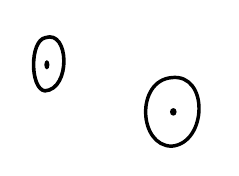
\begin{tikzpicture}[x=.65cm,y=.65cm,line cap=round]
\draw[line width=1.3pt] (0,.06) .. controls (-.29,.10) and (-.30,1.04) .. (.01,1.10) .. controls (.48,1.26) and (.51,.09) .. (0,.06);
\fill (.04,.57) ellipse (.05 and .09);
\draw[line width=1.25pt] (2.48,-1.02) .. controls (1.83,-1.02) and (1.77,.26) .. (2.48,.32) .. controls (3.21,.40) and (3.17,-.96) .. (2.48,-1.02);
\fill (2.51,-.35) ellipse (.065 and .075);
\end{tikzpicture}}
\diagram{\scriptsize\begin{tikzcd}[ampersand replacement=\&,column sep=1.2em,row sep=1em]
{} \& \text{loc. factoriel}\arrow[r,Rightarrow]\arrow[dr,Rightarrow] \& \text{\inserted{loc.} quasi-factoriel}\arrow[r,Rightarrow] \& \text{parafactoriel}\\
\widetilde A\longrightarrow\widetilde A_0 \& {} \& \text{1\unsure{-}factoriel,}\arrow[l]\arrow[d,Rightarrow] \& {}\\
\deleted{\unsure{\widetilde A=}} \& {} \& \text{0-factoriel,} \& {}
\end{tikzcd}}
\[
H^1(X,\underline O_X)=0
\]

$L\qquad L_B$
\figure{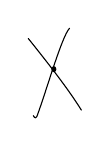
\begin{tikzpicture}[x=.50cm,y=.50cm,line cap=round]
\draw (-.65,.78) .. controls (-.20,.22) and (.36,-.49) .. (.70,-1.04);
\draw (.40,1.04) .. controls (.20,.83) and (-.19,-.56) .. (-.43,-1.20) .. controls (-.47,-1.29) and (-.52,-1.18) .. (-.52,-1.18);
\fill (0,0) ellipse (.065 and .078);
\end{tikzpicture}}
\[
\begin{matrix}\widetilde X\\[.4em]X\end{matrix}
\qquad
\begin{aligned}&\deleted{\unsure{1-d=|1-2=|1\ \text{dim}}}\\ &1-h^1=2-h'-h''\end{aligned}
\]
\[
J\subset A\subseteq B\qquad
\]
\[
\vdots\qquad \underline{A/J\qquad B/JB}
\]
\[
\begin{aligned}
1-g&=\sum(1-g_i)-\sum n_s\quad\unsure{=-}\\
1-g&=\unsure{\nu|v}-\sum g_i-\sum n_s
\end{aligned}
\]
\figure{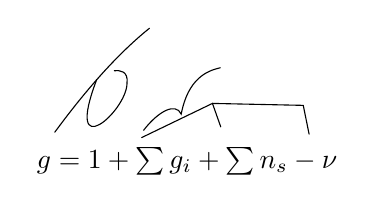
\begin{tikzpicture}[x=.62cm,y=.62cm,line cap=round]
\draw (-1.66,-.08) .. controls (-1.10,.68) and (-.44,1.47) .. (.28,2.05);
\draw (-.80,1.00) .. controls (-1.48,-.78) and (-.19,.34) .. (-.18,.92) .. controls (-.15,1.18) and (-.33,1.19) .. (-.44,1.18);
\draw (.16,-.04) .. controls (.46,.35) and (.82,.54) .. (.93,.29) .. controls (1.07,1.02) and (1.46,1.18) .. (1.73,1.24);
\draw (.12,-.19)--(1.57,.51)--(1.74,.03);
\draw (1.57,.51)--(3.43,.47)--(3.55,-.12);
\node[below] at (1.05,-.19) {$g=1+\sum g_i+\sum n_s-\nu$};
\end{tikzpicture}}
\figure{
\begin{tikzpicture}[x=.47cm,y=.47cm,line cap=round]
\draw[very thick] (0,-.56) .. controls (-.72,-.46) and (-.49,.69) .. (.08,.69) .. controls (.65,.73) and (.66,-.47) .. (0,-.56);
\draw[very thick] (-.01,-.68) .. controls (-.13,-.08) and (.14,.37) .. (.51,.70);
\fill (.08,.01) ellipse (.13 and .12);
\end{tikzpicture}}
\[
\begin{array}{ll}
1-g=1-g'-\sum n_s & 1-g=2-g'-g''-\sum n_s\\[.6em]
g=g'+\sum n_s & g=(g'+g'')+\sum n_s-1
\end{array}
\]
\figure{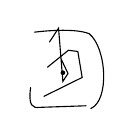
\begin{tikzpicture}[x=.50cm,y=.50cm,line cap=round]
\draw (-.88,1.00) .. controls (-.47,1.05) and (.19,1.09) .. (.51,.96) .. controls (.95,.60) and (1.03,-.73) .. (.55,-.94);
\draw (-.98,-.41) .. controls (-1.04,-.88) and (-.93,-.93) .. (-.75,-.91)--(.43,-.87);
\draw (-.64,-.63)--(.33,-.15)--(.22,.51)--(-.02,.54)--(-.55,.11);
\draw (-.50,.75)--(-.27,1.10)--(-.16,-.25)--(-.03,-.05)--(-.20,.31);
\fill (-.16,-.03) circle (.06);
\end{tikzpicture}}
\[
k[\unsure{x|u},y,z]/xy
\]
\figure{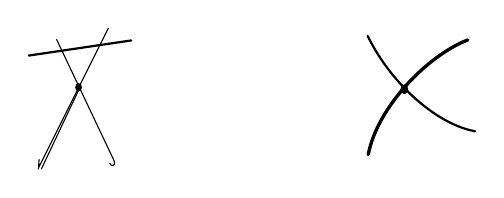
\begin{tikzpicture}[x=.62cm,y=.62cm,line cap=round]
\draw[thick] (-1.04,.67)--(1.06,.98);
\draw (-.47,1.00)--(.71,-1.49) .. controls (.74,-1.62) and (.64,-1.59) .. (.62,-1.54);
\draw (.59,1.23)--(-.84,-1.63)--(-.83,-1.46);
\draw (-.78,-1.65)--(-.02,-.04);
\fill (-.02,.02) ellipse (.07 and .085);
\begin{scope}[xshift=4.1cm]
\draw[thick] (-.71,1.07) .. controls (-.21,.05) and (.74,-.75) .. (1.49,-.88);
\draw[very thick] (-.70,-1.36) .. controls (-.51,-.37) and (.53,.68) .. (1.34,.99);
\fill (.04,-.02) ellipse (.08 and .10);
\end{scope}
\end{tikzpicture}}
\[
\deleted{g'+g''}\qquad g'=g''=0\qquad\sum g_i
\]
% archive sheet number: 65
